\section{Algoritmo}

// TODO: ...

\subsection{Simulazione}
Viene di seguito mostrato un esempio di funzionamento per via dei messaggi di log sulla console
\subsubsection{Setup:}
Per questa simulazione si sono scelti i seguenti valori:
\begin{itemize}
	\item Producer: sleep ogni 500 millisecondi;
	\item Consumer: sleep ogni 2 secondi;
	\item Checker: sleep ogni 3 secondi;
	\item Cliente: 4 thread con sleep random tra 10 e 60 secondi;
	\item Cuoco: 4 thread con sleep in base all'ordine variabile tra 10 e 60 secondi;
	\item Buffer size: 10 posti;
	\item Buffer cucina: 10 posti (numero di ordini totali in cucina);
	\item Capacità singola coda postazione: 5 posti;
	\item 4 Code di postazione: PASTA, RISO, CARNE, PESCE.
\end{itemize}
\subsubsection{Cliente e Producer:}
\begin{figure}[H]
	\centering
	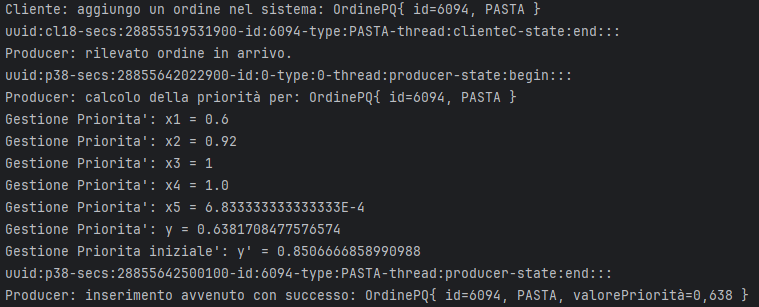
\includegraphics[scale=0.75]{iterazione3/images/Cliente-Producer.png}
	\caption{Funzionamento Thread Cliente e Producer \label{fig:Cliente-Producer}}
\end{figure}
In Figura\vref{fig:Cliente-Producer} è mostrata l'interazione tra il thread Cliente e il Producer, si può notare come il Cliente effettua un'ordinazione aggiungendo un ordine nel sistema, viene mostrato l'id dell'ordine e il tipo di ingrediente principale, successivamente il Producer si attiva e rileva un ordine all'interno della sua coda, prende questo ordine, gli calcola una priorità passando per la classe Gestione Priorità, e lo inserisce nel buffer. Vengono inoltre mostrati sulla console i passi che si compiono per calcolare la priorità. La priorità iniziale $y'$ differisce dalla $y$ poiché è calcolata senza il contributo del parametro $x5$ visto che nullo all'entrata nel buffer (quindi viene calcolata facendo la somma pesata solo dei primi 4 parametri).
\subsubsection{Checker:}
\begin{figure}[H]
	\centering
	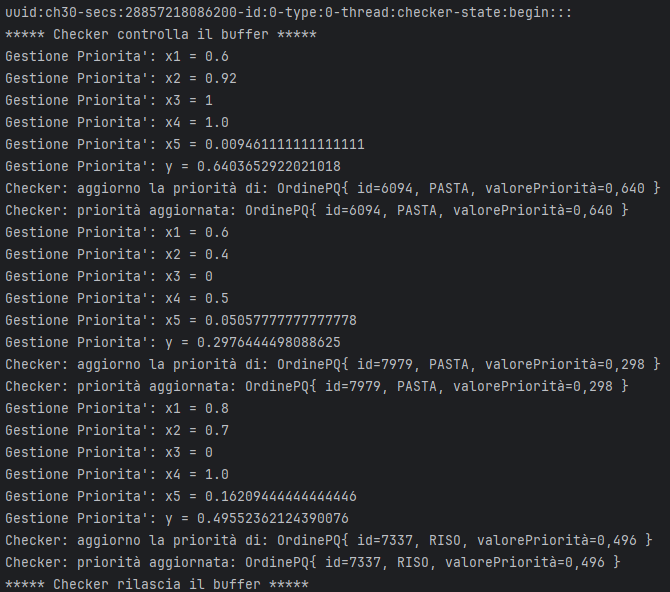
\includegraphics[scale=0.75]{iterazione3/images/Checker.png}
	\caption{Funzionamento Thread Checker \label{fig:Checker}}
\end{figure}
In Figura\vref{fig:Checker} è mostrato il comportamento del Checker, il quale si attiva, controlla in maniera mutualmente esclusiva il buffer e seleziona tramite una finestra mobile gli ordini da controllare ed aggiornare la priorità. Ogni aggiornamento di priorità è seguito da un aggiornamento del buffer im modo da riportare la modifica appena apportata all'ordine.
\subsubsection{Consumer e Producer:}
\begin{figure}[H]
	\centering
	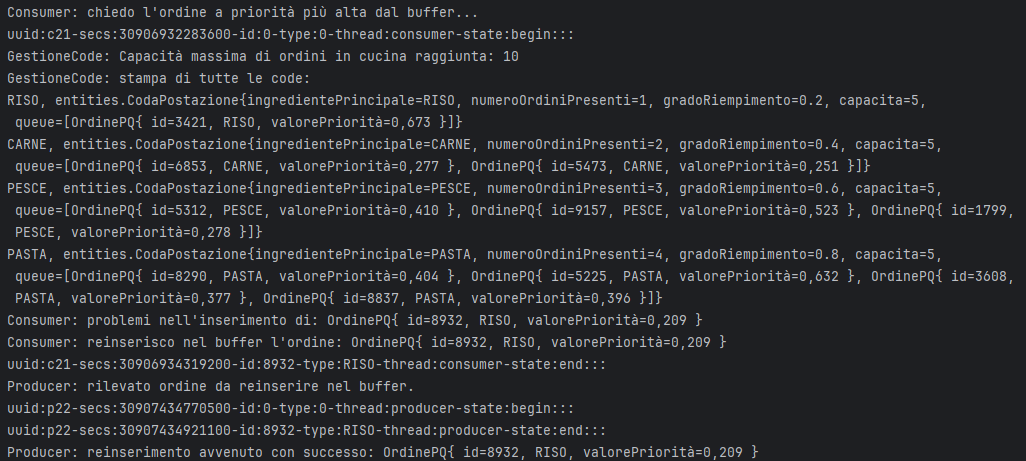
\includegraphics[scale=0.5]{iterazione3/images/consumer-producer.png}
	\caption{Funzionamento Thread Consumer e Producer \label{fig:consumer-producer}}
\end{figure}
In Figura\vref{fig:consumer-producer} è mostrato il caso in cui il Consumer estrae l'ordine a priorità più elevata dal buffer ma non può inviarlo in cucina poiché è stato raggiunto il numero massimo di ordini che possono esistere contemporaneamente in cucina, per questo motivo lo passa al Producer per poterlo reinserire all'interno del buffer. Viene stampato lo stato di ogni coda di postazione per una verifica (infatti si nota che la somma degli ordini in cucina è 10 come segnalato). Il Producer riceve quindi l'ordine e lo reinserisce immediatamente nel buffer.
\subsubsection{Consumer:}
\begin{figure}[H]
	\centering
	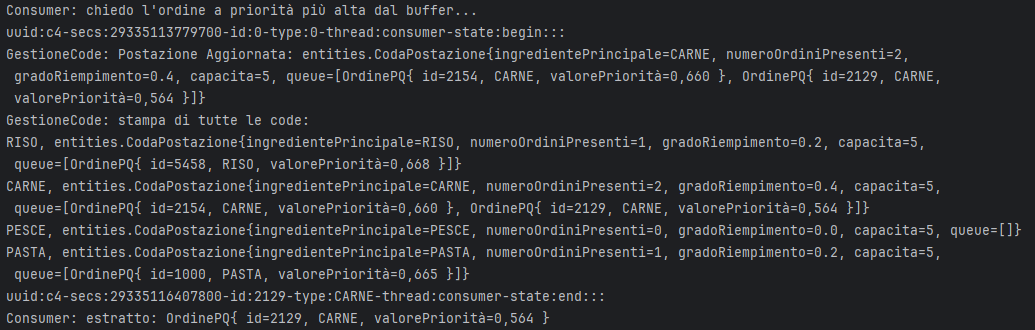
\includegraphics[scale=0.5]{iterazione3/images/Consumer.png}
	\caption{Funzionamento Thread Consumer \label{fig:Consumer}}
\end{figure}
In Figura\vref{fig:Consumer} è mostrato il caso di funzionamento ordinale del Consumer, cioè il caso in cui estrae l'ordine a priorità più elevata dal buffer e lo inserisce nella corrispettiva coda di postazione per ingrediente principale in cucina. Anche in questo caso viene stampato lo stato di ogni coda di postazione per una semplice verifica.
\subsubsection{Cuoco:}
\begin{figure}[H]
	\centering
	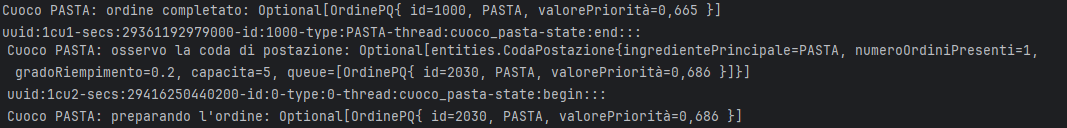
\includegraphics[scale=0.5]{iterazione3/images/Cuoco.png}
	\caption{Funzionamento Thread Cuoco \label{fig:Cuoco}}
\end{figure}
In Figura\vref{fig:Cuoco} è mostro il lavoro del cuoco, nello specifico quello adibito alla postazione dell'ingrediente principale PASTA, il quale finisce di preparare un ordine, invia di conseguenza una notifica di avvenuta preparazione e si mette in attesa sulla propria coda di postazione, rileva quindi un ordine in coda e comincia la preparazione quel nuovo ordine rilevato.
\subsubsection{Dati simulazione:}
Per quanto riguarda i dati della simulazione e l'analisi di questi per valutare la performance dell'algoritmo si fa riferimento alla sezione \vref{sec:analDati}.
\clearpage